\chapter{Aprendizaje de política basado en modelo}%
\label{cha:aprendizaje_de_política_basado_en_modelo}

\lecture{13}{2020-07-02}{Model Based Policy Learning}

En el tema 9 se habló de algoritmos basado en modelo en los que se planificaban las
acciones y por tanto no había política. En este tema se usan políticas. Se tratarán tanto
políticas globales (las normales de siempre) y las políticas locales (políticas que solo
aproximan valores correctos en un subconjunto de estados).

En el tema 9 al último algoritmo al que se llegó fue el MPC (página 57).

Si se quiere entrenar un modelo de la dinámica a la vez que una política, ambas representadas
con una red neuronal, se podría pensar que entrenar de esta manera:
\begin{figure}[htpb]
	\centering
	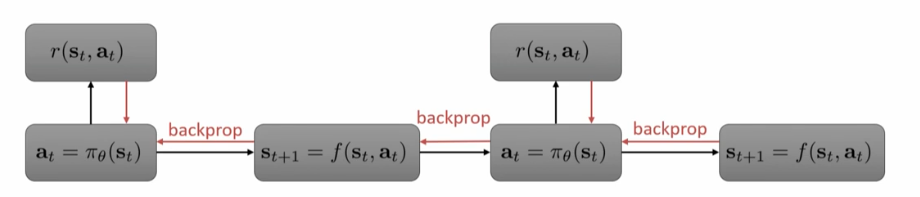
\includegraphics[width=0.8\linewidth]{figures/2020-07-02-162725_920x197_scrot.png}
\end{figure}
fuera una buena idea. Pero tiene el problema que los episodios al poder tener cientos de
pasos aparece el problema de los \textit{vanishing gradient} o \textit{exploding
gradients}. Además, las acciones que se tomen al principio afectarán mucho más a los estados
finales (efecto mariposa) lo que lleva a la inestabilidad numérica (como los \textit{shooting
methods}). Por lo que no se pueden utilizar métodos como LQR. Los problemas son parecidos a los
del entrenamiento de las redes neuronales recurrentes con
\textit{backpropagation}, pero no se puede jugar con los valores propios de las jacobianas ya
que se tienen que aprender las dinámicas del mundo y no se pueden modificar los datos.

Como posibles soluciones:
\begin{itemize}
    \item Se pueden usar algoritmos RL sin derivadas (sin modelo), donde el modelo es usado para
        generar muestras sintéticas. Puede parecer una idea absurda pero en la práctica funciona
        bastante bien. Se puede pensar en ello como una 'aceleración basada en modelo' para
        algoritmos RL sin modelo.
    \item Usar políticas más sencillas que redes neuronales. Por ejemplo: LQR con modelos
        aprendidos (LQR-FLM). Donde se entrenan políticas locales para resolver tareas
        simples. También se puede usar aprendizaje supervisado para combinarlas y
        conseguir una política global.
\end{itemize}

\section{Optimización sin modelo con un modelo}%
\label{sec:optimización_sin_modelo_con_un_modelo}

Mirando a la fórmula de Policy Gradient:
\begin{align}
\nabla _ { \theta } J ( \theta ) \approx \frac { 1 } { N } \sum _ { i = 1 } ^ { N } \sum _ { t = 1 } ^ { T } \nabla _ { \theta } \operatorname { log } \pi _ { \theta } ( a _ { i , t } | s _ { i , t } ) \hat { Q } _ { i , t } ^ { \pi }
\end{align}
Es peculiar ver que no hace falta hacer ninguna regla de la cadena pero aún así Policy Gradients
optimiza a través del tiempo. La clave está en que es la derivada de una esperanza. El
gradiente de la retropropagación del camino se expresa como:
\begin{align}
\nabla _ { \theta } J ( \theta ) = \sum _ { t = 1 } ^ { T } \frac { d r _ { t } } { d s _ { t } } \prod _ { t ^ { \prime } = 2 } ^ { t } \frac { d s _ { t ^ { \prime } } } { d a _ { t ^ { \prime } - 1 } } \frac { d a _ { t ^ { \prime } - 1 } } { d s _ { t ^ { \prime } - 1 } }
\end{align}
Esto es un poco inútil. Pero con el truco de la reparametrización del tema anterior aplicada a
esta ecuación en entornos estocásticos, calcula el mismo gradiente que Policy Gradient,
pero de una manera diferente, por lo que hay ventajas y desventajas para cada uno. PG tiene
una alta varianza y BT no tiene ese problema pero para episodios largos es más probable que la
aproximación numérica no sea buena. 

Si se tuviera un modelo del entorno, se podrían generar millones de muestras y reducir así la
varianza de PG. Por lo que PG se vuelve más estable ya que no hay que multiplicar ninguna
serie jacobiana.

En la publicación: 
\textit{ Parmas et al. '18: PIPP: Flexible Model-Based Policy Search Robust to the Curse of Chaos, }
dicen que aunque se pueda usar BT, suele ser preferible usar PG.

Este método (usando PG) también tiene sus problemas cuando los episodios son largos. Estos vienen
de que el modelo del entorno no es perfecto y va introduciendo errores que se van acumulando y
hacen que los datos producidos al final no valgan. Lo que hace que la estimación de PG no
sea buena.

Aquí es donde entran los métodos 'Dyna'. Consiste en un algoritmo Online Q-Learning que hace RL
sin modelo con un modelo.

\begin{algorithm}
    \caption{Dyna}
    Dado el estado $s$, escoger una acción $a$ usando la política exploratoria\\
    Observar $s'$ y $r$, obtener la transición $(s,a,s',r)$.\\
    Actualizar el modelo $\hat{p}(s'|s,a)$ y $\hat{r}(s,a)$ usando $(s,a,s')$ \\
    Actualización de Q: $Q(s,a)\gets Q(s,a)+\alpha E_{s',r}[r+\max_{a'}Q(s',a')-Q(s,a)]$\\
    \Repeat{K veces}{
        Muestrear $(s,a)\sim B$ del buffer de acciones y estados pasados\\
        Actualización de Q: $Q(s,a)\gets Q(s,a)+\alpha E_{s',r}[r+\max_{a'}Q(s',a')-Q(s,a)]$\\
    }
\end{algorithm}

El modelo se usa para calcular las esperanzas. Este es el algoritmo propuesto en el
paper original por R. Sutton. Hoy en día la generalización del algoritmo que se suele usar es la
siguiente:

\begin{algorithm}
    \caption{Dyna Generalizado}
    Recolectar algunos datos, consistiendo en las transiciciones $(s,a,s',r)$\\
    Aprender el modelo  $\hat{p}(s'|s,a)$ (y opcionalmente $\hat{r}(s,a)$).\\
    \Repeat{K veces}{
        Muestrear $s\sim B$ del buffer\\
        Elegir la acción $a$ (de $B$, a partir de $\pi$ o aleatoriamente)\\
        Simular $s'\sim \hat{p}(s'|s,a)$ (y $r=\hat{r}(s,a)$)\\
        Entrenar sobre $(s,a,s',r)$ el algoritmo RL sin modelo\\
        (Opcionalmente) tomar $N$ pasos más con el modelo.
    }
\end{algorithm}

Las ventajas de este método son:
\begin{itemize}
    \item Los \textit{rollouts} no tienen por qué ser muy grandes. Normalmente con
        $N=1$ está bien.
    \item Se exploran estados diversos.
\end{itemize}

\begin{figure}[H]
	\centering
	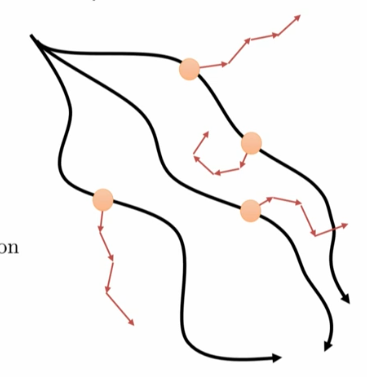
\includegraphics[width=0.3\linewidth]{figures/2020-07-02-172155_367x377_scrot.png}
\end{figure}

Como desventajas de estos métodos, es difícil saber cuando usarlos es mejor que usar algoritmos
sin modelo. Además si el modelo es malo se tienen actualizaciones malas.

\section{Modelos locales}%
\label{sec:modelos_locales}

Cuando se habló de control óptimo, se vió que se puede reescribir el problema de control
como una optimización sin restricciones.
\begin{align}
\operatorname { min } _ { u _ { 1 } , \ldots , u _ { T } } \sum _ { t = 1 } ^ { T } c ( x _ { t }
, u _ { t } ) \text { s.t. } x _ { t } = f ( x _ { t - 1 } , u _ { t - 1 } )\\
\operatorname { min } _ { u _ { 1 } , \ldots , u _ { T } } c ( x _ { 1 } , u _ { 1 } ) + c ( f ( x _ { 1 } , u _ { 1 } ) , u _ { 2 } ) + \cdots + c ( f ( f ( \ldots ) \ldots ) , u _ { T } )
\end{align}

Donde se necesita $\frac{df}{dx_t},\frac{df}{du_t},\frac{dc}{dx_t},\frac{dc}{du_t}$. En
RL, no se tiene el conocimiento de las primeras dos de estas derivadas. Por lo que si se
aprendiese un modelo para poder calcular las derivadas sobre ese modelo, se podría entonces
utilizar algoritmos como LQR y obtener políticas locales.

La idea es sencilla: se tiene una política y con suerte las trayectorias que produce están cerca
las unas de las otras, por lo que se pueden coger esas trayectorias y ajustar una dinámica
lineal (regresión lineal) para cada paso del tiempo.

El procedimiento es ejecutar el controlador para conseguir unas trayectorias y ajustar las
dinámicas:
\begin{figure}[H]
	\centering
	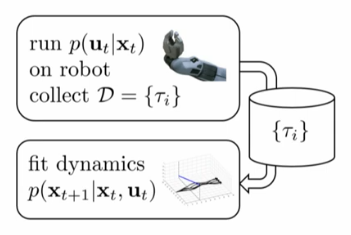
\includegraphics[width=0.3\linewidth]{figures/2020-07-02-173627_351x235_scrot.png}
\end{figure}
Las dinámicas serán unas gaussianas condicionadas:
\begin{align}
p ( x _ { t + 1 } | x _ { t } , u _ { t } ) = N ( f ( x _ { t } , u _ { t } ) , \Sigma )
\end{align}
La media de esas gaussianas es una función lineal.
\begin{align}
f ( x _ { t } , u _ { t } ) \approx A _ { t } x _ { t } + B _ { t } u _ { t }
\end{align}
$\Sigma$ no hace falta aproximarla ya que no afecta a LQR. Con esto, se tiene:
\begin{align}
A _ { t } = \frac { d f } { d x _ { t } } \quad B _ { t } = \frac { d f } { d u _ { t } }
\end{align}
Se mejora el controlador y se repite el proceso.

Para formular un algoritmo práctico de este tipo se tiene que resolver la pregunta de qué
controlador se tiene que ejecutar.

iLQR produce $\hat{x}_t,\hat{u}_t, K_t,k_t$, y:
\begin{align}
    u_t=K_t(x_t= \hat{x}_t)+k_t+\hat{u}_t
\end{align}
Se puede pensar que una acción de control razonable sería
$p(u_t|x_t)=\delta(u_t=\hat{u}_t)$. Pero esto no corrige ni las desviaciones ni la deriva. Por lo
que en su lugar se puede pensar en coger:
\begin{align}
p ( u _ { t } | x _ { t } ) = \delta ( u _ { t } = K _ { t } ( x _ { t } - \hat { x } _ { t } ) + k _ { t } + \hat { u } _ { t } )
\end{align}
Donde $K_t$ sirve para compensar los pequeños errores del modelo. Pero la aproximación lineal
puede ser un problema al ser demasiado mala en el caso de que todas las trayectorias sean
muy parecidas o estén muy dispersas. 

Una mejor elección sería construir un controlador estocástico tal que:
\begin{align}
p ( u _ { t } | x _ { t } ) = N ( K _ { t } ( x _ { t } - \hat { x } _ { t } ) + k _ { t } + \hat { u } _ { t } , \Sigma _ { t } )
\end{align}
Una buena elección de $\Sigma_t$ es $\Sigma_t=Q^{-1}_{u_t,u_t}$. Una intuición de esto es
que  $Q$ modela la curvatura local de la función $Q$. Por lo que en curvaturas agudas no
se quiere una varianza alta y viceversa.

¿Cómo se aprenden las dinámicas (A y B)? Con regresión lineal se tiene el problema de que los
datos requeridos crecen con la dimensionalidad del problema. En la práctica esto se puede
simplificar usando \textbf{regresión lineal bayesiana} usando nuestro modelo global favorito (red
neuronal, mezcla de gaussianas, \ldots) como el conocimiento a priori.

¿Qué pasa si nos vamos muy lejos? Como la aproximación es lineal, si nos alejamos de la
aproximación el controlador tomará acciones malas y este error se acentuará en estados futuros.
\begin{figure}[H]
	\centering
	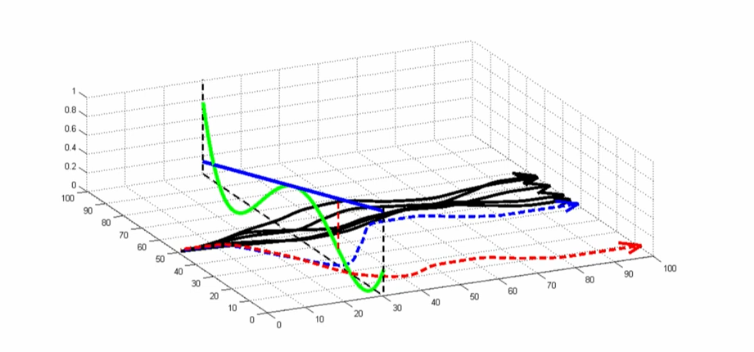
\includegraphics[width=0.6\linewidth]{figures/2020-07-02-185253_754x352_scrot.png}
\end{figure}

Para que este método funcione bien, se tiene que conseguir que la nueva distribución de
trayectorias $p(\tau)$ esté cerca de la distribución anterior
$\overline{p}(\tau)$. Tal como se vio en TRPO donde se restringía la divergencia KL para
mantener las distribuciones similares entre sí, aquí se va a hacer lo mismo. Ya que si las
trayectorias son similares, las dinámicas también lo serán. Que las distribuciones estén
cerca significa que $D_{KL}(p(\tau)||\overline{p}(\tau))\leq\epsilon$. Resulta que esto es
muy fácil de hacer si $\overline{p}(\tau)$ vino también de un controlador lineal.

Para más detalles, mirar el paper: \textit{ Learning Neural Network Policies with Guided Policy Search under Unknown Dynamics }

\section{Combinar modelos locales en un modelo global}%
\label{sec:combinar_modelos_locales_en_un_modelo_global}

Se le llama búsqueda de política guiada. Consiste en generar varias trayectorias con
algoritmos sencillos basados en modelo como por ejemplo iLQR y con todas las muestras obtenidas
entrenar una red neuronal para que reproduzca el modelo. Esto funciona bien pero se puede mejorar
si una vez se ha entrenado la red se modifican los controladores LQR para que intenten
aproximarse a la política global de la red neuronal. Esto hace que los diversos
controladores lleguen a un consenso y se converja a una política global buena.

\begin{algorithm}
    \caption{Búsqueda guiada de política}
    \Repeat{}{
        Optimizar cada política global $\pi_{LQR,i}(u_t|x_t)$ en el estado inicial $x_{0,i}$ 
        con respecto a $\tilde{c}_{k,i}(x_t,u_t)$.\\
        Usar las muestras del paso anterior para entrenar $\pi_\theta$ de forma que mimetice cada
        $\pi_{LQR,i}(u_t|x_t)$\\
        Actualizar la función de coste $ \tilde { c } _ { k + 1 , i } ( x _ { t } , u _ { t } ) =  c (
        x _ { t } , u _ { t } ) - \lambda _ { k + 1 , i } \operatorname { log } \pi _ { \theta } ( u
        _ { t } | x _ { t } ) $
    }
\end{algorithm}

El coste $\tilde{c}_{k,i}$ será modificado levemente para mantener $\pi_{LQR,i}$ cerca de
$\pi_\theta$. $\lambda_{k+1,i}$ puede ser visto como un multiplicador de Lagrange para la
restricción que se asegura que en la convergencia $\pi_\theta$ hace lo mismo que $\pi_{LQR}$.

\begin{figure}[H]
	\centering
	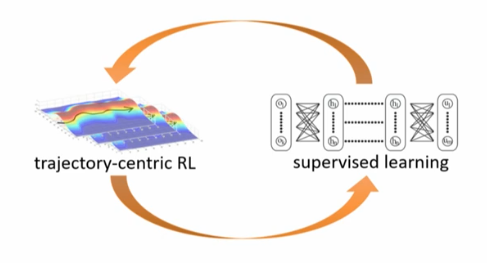
\includegraphics[width=0.6\linewidth]{figures/2020-07-02-192432_487x263_scrot.png}
\end{figure}

Esta idea puede ser utilizada en otros ámbitos de RL, como por ejemplo RL sin modelo, o en
ámbitos fuera de RL como por ejemplo la técnica de la destilación
(\textit{distillation}).

Esta técnica viene del mundo del aprendizaje supervisado para entrenar redes neuronales. La
técnica se aplica para evitar los \textbf{ensemble models}: que consiste en entrenar varios modelos y calcular
la media de sus predicciones, en vez de tener solamente un modelo con una única predicción.

La técnica de la destilación se basa en entrenar un modelo sobre las predicciones de los
otros modelos como 'objetivos blandos' (\textit{soft-targets}). La idea está en que los
\textit{labels} del aprendizaje supervisado no dan mucha información. Por ejemplo en MNIST
pueden haber números que estén mal escritos y se parezcan a otros, por lo que los modelos no
estarán 100\% seguros de su decisión aunque el \textit{label} es 100\% cierto.

La extensión a RL se llama \textit{Distillation for Multi-Task Transfer}. Era una publicación
en la que se pretendía tener un agente que jugase a todos los juegos de Atari. Se entrena un
agente por cada juego y luego se crea otro agente que los engloba a todos usando aprendizaje
supervisado y destilación.

Otra técnica diferente a la destilación es la de 'divide y vencerás', en la cual en vez de tener
algoritmos LQR para las políticas locales se tienen más redes neuronales. Un sketch del algoritmo
sería
\begin{algorithm}
    \caption{Divide and conquer RL}
    \Repeat{}{
        Optimizar cada política local $\pi_{\theta_i}(a_t|s_t)$ sobre los estados iniciales
        $s_{0,i}$ con respecto a $\tilde{r}_{k,i}(s_t,a_t)$.\\
        Usar las muestras del paso anterior para entrenar $\pi_\theta(a_t|x_t)$ para mimetizar cada
        $\pi_{\theta_i}(a_t|s_t)$.\\
        Actualizar la función de recompensa $ \tilde { r } _ { k + 1 , i } ( x _ { t } , u _ { t } )
        = r ( x _ { t } , u _ { t } ) + \lambda _ { k + 1 , i } \operatorname { log } \pi _ { \theta
        } ( u _ { t } | x _ { t } ) $\\
    }
\end{algorithm}

Publicaciones relacionadas:
\begin{itemize}
    \item L. \( ^{*}, \) Finn \( ^{*} \), et al. End-to-End Training of Deep Visuomotor Policies. 2015.
    \item Rusu et al. Policy Distillation. 2015.
    \item Parisotto et al. Actor-Mimic: Deep Multitask and Transfer Reinforcement Learning. 2015. 
    \item Ghosh et al. Divide-and-Conquer Reinforcement Learning. 2017. 
    \item Teh et al. Distral: Robust Multitask Reinforcement Learning. 2017.
\end{itemize}
